\documentclass[11pt]{article} 
\usepackage[english]{babel}
\usepackage[utf8]{inputenc}
\usepackage[margin=0.5in]{geometry}
\usepackage{amsmath}
\usepackage{amsthm}
\usepackage{amsfonts}
\usepackage{amssymb}
\usepackage[usenames,dvipsnames]{xcolor}
\usepackage{graphicx}
\usepackage[colorinlistoftodos, color=orange!50]{todonotes}
\usepackage{hyperref}
\usepackage[numbers, square]{natbib}
\usepackage{fancybox}
\usepackage{epsfig}
\usepackage{soul}
\usepackage[framemethod=tikz]{mdframed}
\usepackage[shortlabels]{enumitem}
\usepackage[version=4]{mhchem}
\usepackage{multicol}
\usepackage{forest}
\usepackage{mathtools}
\usepackage{comment}
\usepackage{enumitem}
\usepackage[utf8]{inputenc}
\usepackage{listings}
\usepackage{color}
\usepackage[numbers]{natbib}
\usepackage{subfiles}
\usepackage{algorithm}
\usepackage[noend]{algpseudocode}


\newtheorem{prop}{Proposition}[section]
\newtheorem{thm}{Theorem}[section]
\newtheorem{lemma}{Lemma}[section]
\newtheorem{cor}{Corollary}[prop]

\theoremstyle{definition}
\newtheorem{definition}{Definition}

\theoremstyle{definition}
\newtheorem{required}{Problem}
\newtheorem*{requiredHC}{Problem HC}

\theoremstyle{definition}
\newtheorem{ex}{Example}

\newcommand{\interval}[4]{\draw (#2, #1) -- (#3, #1); % Usage: \interval{height}{start}{end}{label}
\draw (#2, #1-0.11) -- (#2, #1+0.11); % draw left whisker
\draw (#3, #1-0.11) -- (#3, #1+0.11); % draw right whisker
\node[] at (#2-0.25, #1) {#4};
}


\setlength{\marginparwidth}{3.4cm}
%#########################################################

%To use symbols for footnotes
\renewcommand*{\thefootnote}{\fnsymbol{footnote}}
%To change footnotes back to numbers uncomment the following line
%\renewcommand*{\thefootnote}{\arabic{footnote}}

% Enable this command to adjust line spacing for inline math equations.
% \everymath{\displaystyle}

% _______ _____ _______ _      ______ 
%|__   __|_   _|__   __| |    |  ____|
%   | |    | |    | |  | |    | |__   
%   | |    | |    | |  | |    |  __|  
%   | |   _| |_   | |  | |____| |____ 
%   |_|  |_____|  |_|  |______|______|
%%%%%%%%%%%%%%%%%%%%%%%%%%%%%%%%%%%%%%%

\title{
\normalfont \normalsize 
\textsc{CSCI 3104 Spring 2022 \\ 
Instructor: Profs. Chen and Layer} \\
[10pt] 
\rule{\linewidth}{0.5pt} \\[6pt] 
\huge Problem Set 6 \\
\rule{\linewidth}{2pt}  \\[10pt]
}
%\author{Your Name}
\date{}

\begin{document}
\definecolor {processblue}{cmyk}{0.96,0,0,0}
\maketitle


%%%%%%%%%%%%%%%%%%%%%%%%%
%%%%%%%%%%%%%%%%%%%%%%%%%%
%%%%%%%%%%FILL IN YOUR NAME%%%%%%%
%%%%%%%%%%AND STUDENT ID%%%%%%%%
%%%%%%%%%%%%%%%%%%%%%%%%%%
\noindent
Due Date \dotfill March 8 \\
Name \dotfill \textbf{Julia Troni} \\
Student ID \dotfill \textbf{109280095} \\
Collaborators \dotfill \textbf{Null}

\tableofcontents

\section*{Instructions}
\addcontentsline{toc}{section}{Instructions}
 \begin{itemize}
	\item The solutions \textbf{must be typed}, using proper mathematical notation. We cannot accept hand-written solutions. Useful links and references on \LaTeX can be found \href{https://canvas.colorado.edu/courses/75824/pages/latex}{here on Canvas}.
	\item You should submit your work through the \textbf{class Canvas page} only. Please submit one PDF file, compiled using this \LaTeX \ template.
	\item You may not need a full page for your solutions; pagebreaks are there to help Gradescope automatically find where each problem is. Even if you do not attempt every problem, please submit this document with no fewer pages than the blank template (or Gradescope has issues with it).

	\item You are welcome and encouraged to collaborate with your classmates, as well as consult outside resources. You must \textbf{cite your sources in this document.} \textbf{Copying from any source is an Honor Code violation. Furthermore, all submissions must be in your own words and reflect your understanding of the material.} If there is any confusion about this policy, it is your responsibility to clarify before the due date. 

	\item Posting to \textbf{any} service including, but not limited to Chegg, Reddit, StackExchange, etc., for help on an assignment is a violation of the Honor Code.
\end{itemize}



\newpage
\section{Standard 17: Balanced versus unbalanced partitioning.}

\begin{required}
\subsection{Problem 1}
\begin{enumerate}[label=(\alph*)]
\item \label{(a).}~Consider a modified Merge-Sort algorithm that at each recursion splits an array of size $n$  into two subarrays of sizes $4$ and $n-4$, respectively. Write down a recurrence relation for this modified Merge-Sort algorithm and give its asymptotic solution.

\begin{proof}[Answer]
% YOUR ANSWER HERE
\begin{align*}
T(n) = \begin{cases}
\Theta(1) & : n \leq 5, \\
4+T(n - 4) + \Theta(n) & : n > 5.
\end{cases}
\end{align*}

Using loop unrolling:
\begin{align*}
T(n) &= T(n-4)+4+cn\\
&= T(n-8)+c(n-4)+cn + 2\cdot4 \\
&= T(n-12) + c(n-8)+c(n-4)+cn + 3\cdot4 \\
&= T(n-16)+ c(n-12) + c(n-8)+c(n-4)+cn + 4\cdot4 \\
&... \\
						&=T(n-4k)+c\cdot \sum_{i=0}^{k}(n-4i) + k\cdot4
\end{align*}
To find the number of times we need to unroll, we know we hit the base case when $n-4k <5$\\
So solve for $k$ to get : $k>\frac{n-5}{4}$\\
So we unroll until $k = \lceil\frac{n-5}{4} \rceil$ \\
Thus we have that: \\
\begin{align*}
T(n) &=T(n-4\cdot\lceil\frac{n-5}{4} \rceil)+c\cdot\sum_{i=0}^{\lceil\frac{n-5}{4} \rceil}(n-4i) + \cdot\lceil\frac{n-5}{4} \rceil \cdot 4 + 4\cdot\lceil\frac{n-5}{4} \rceil \\
&=\Theta(1)+cn \cdot \lceil\frac{n-5}{4} \rceil - \frac {4c\lceil\frac{n-5}{4} \rceil\cdot (\lceil\frac{n-5}{4} \rceil +1) } {2}  + 4\cdot\lceil\frac{n-5}{4} \rceil \\
&=\Theta(1)+cn\cdot \lceil\frac{n-5}{4} \rceil - 2c\lceil\frac{n-5}{4} \rceil\cdot (\lceil\frac{n-5}{4} \rceil +1) +  4\cdot\lceil\frac{n-5}{4} \rceil 
\end{align*}
Thus we have that $T(n) \in \Theta(n^2)$

\end{proof}
\newpage

\item \label{(b)}~Consider a modified Merge-Sort algorithm that at each recursion splits an array of size $n$  into two subarrays of sizes $\frac{1}{5}n$ and $\frac{4}{5}n$, respectively. Write down a recurrence relation for this modified Merge-Sort algorithm and give its asymptotic solution.


\begin{proof}[Answer]
% YOUR ANSWER HERE
\begin{align*}
T(n) = \begin{cases}
\Theta(1) & : n \leq 5, \\
T(\frac{n}{5}) + T(\frac{4n}{5} + \Theta(n) & : n > 5.
\end{cases}
\end{align*}

The tree is depicted below \\
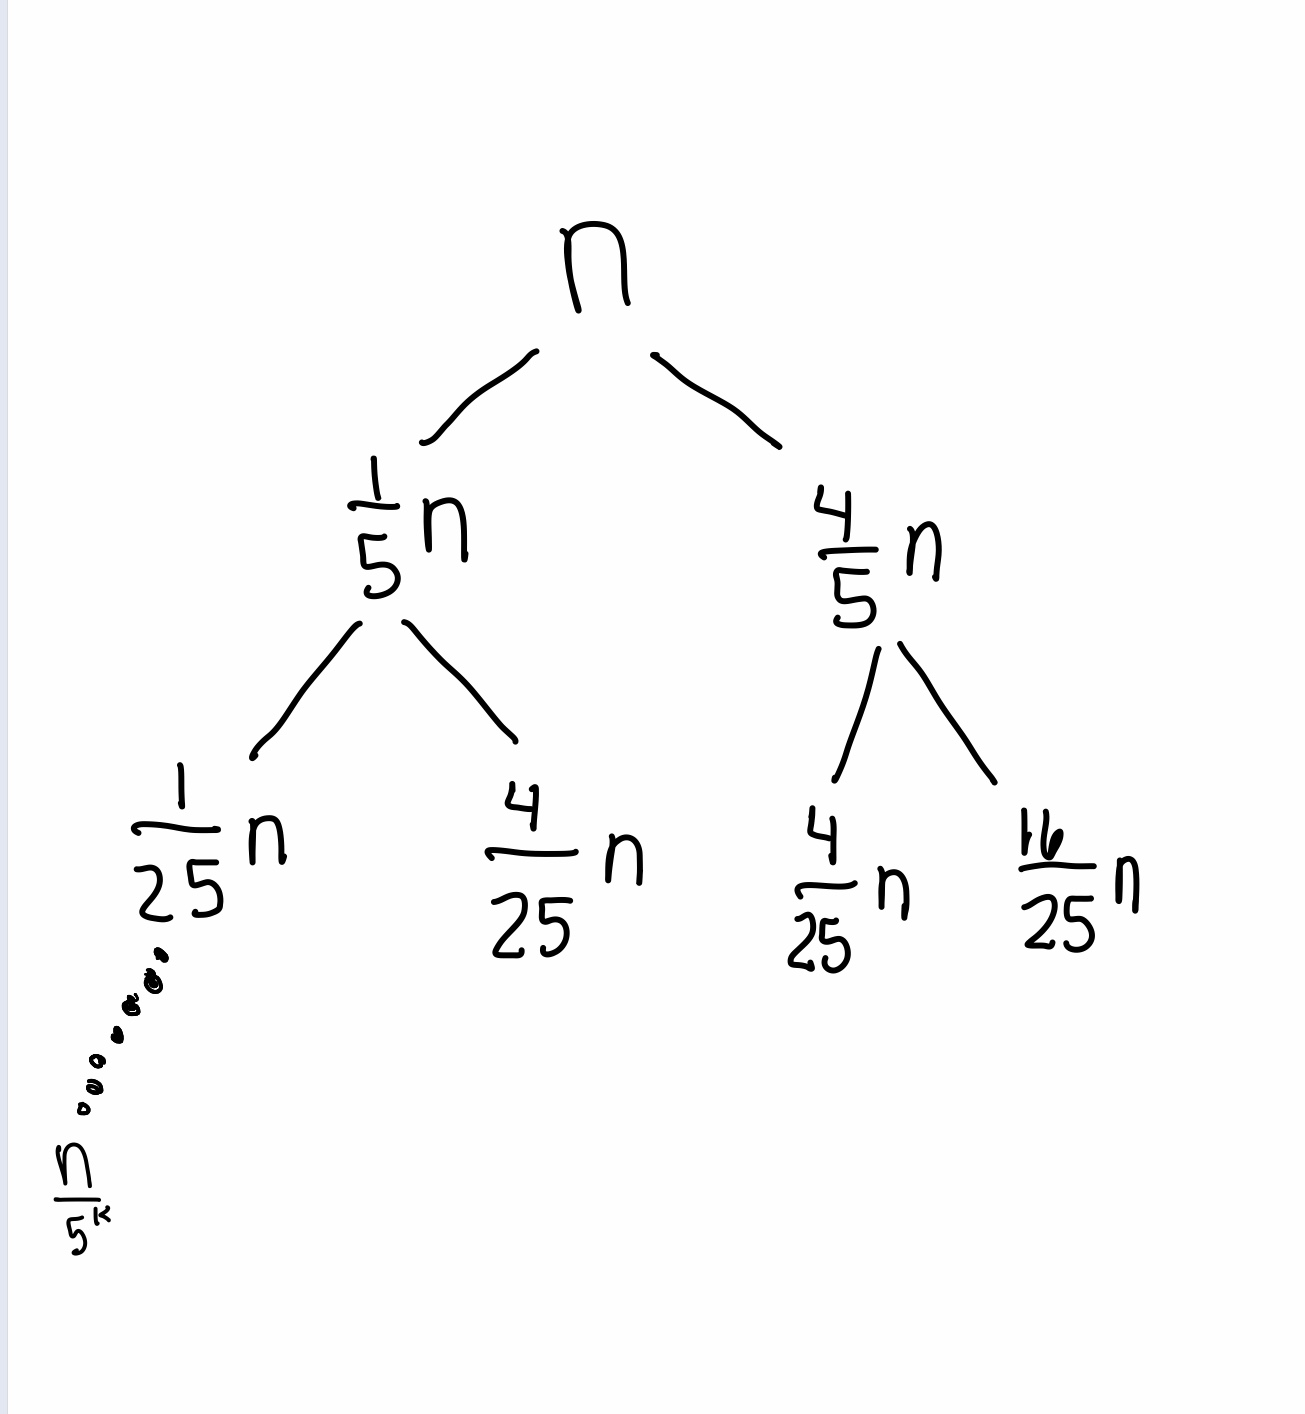
\includegraphics[width=0.5\textwidth]{1bHw6}


Note that the cost at each level (as long as no branches have reached their base case) is n. Thus we do at most $O(n)$ work in each layer\\
The upper bound of the number of possible layers is the depth of the deepest base case path. The largest recursion at each level is $\frac{n}{5}$, so the longest depth of the tree will occur when we reach base case for the $T(\frac{n}{5}) $ term. \\
We hit that base case when $ \frac{n}{5^k}\leq5$\\
So solve for $k$ to get : $k\geq log_{5}n -1$\\
So the path must terminate by depth $k = \lceil\ log_{5}n -1 \rceil$ \\
Thus the total run time is $T(n) \leq n \cdot \lceil\ log_{5}n -1 \rceil$ \\


Thus we have that $T(n) \in O(nlog_5n)$
\end{proof}


\newpage

\item \label{(c)}~Suppose that we modify the Merge-Sort algorithm in such a way that on alternating levels of the recursion, the partitioning is either a $(2, n-2)$ split or a $(n/2,~n/2)$ split. Write down a recurrence relation for this modified Merge-Sort algorithm and give its asymptotic solution. Then, give a verbal explanation of how this Merge-Sort algorithm changes the running time of Merge-Sort.


\begin{proof}[Answer]
% YOUR ANSWER HERE
The recurrences are \\
\begin{align*}
T_1(n) = \begin{cases}
\Theta(1) & : n \leq 2, \\
T_2(n-2) + 2+ \Theta(n) & : n > 2.
\end{cases}
\end{align*}
\begin{align*}
T_2(n) = \begin{cases}
\Theta(1) & : n \leq 2, \\
2T_1(\frac{n}{2}) + \Theta(n) & : n > 2.
\end{cases}
\end{align*}

The tree is below: \\
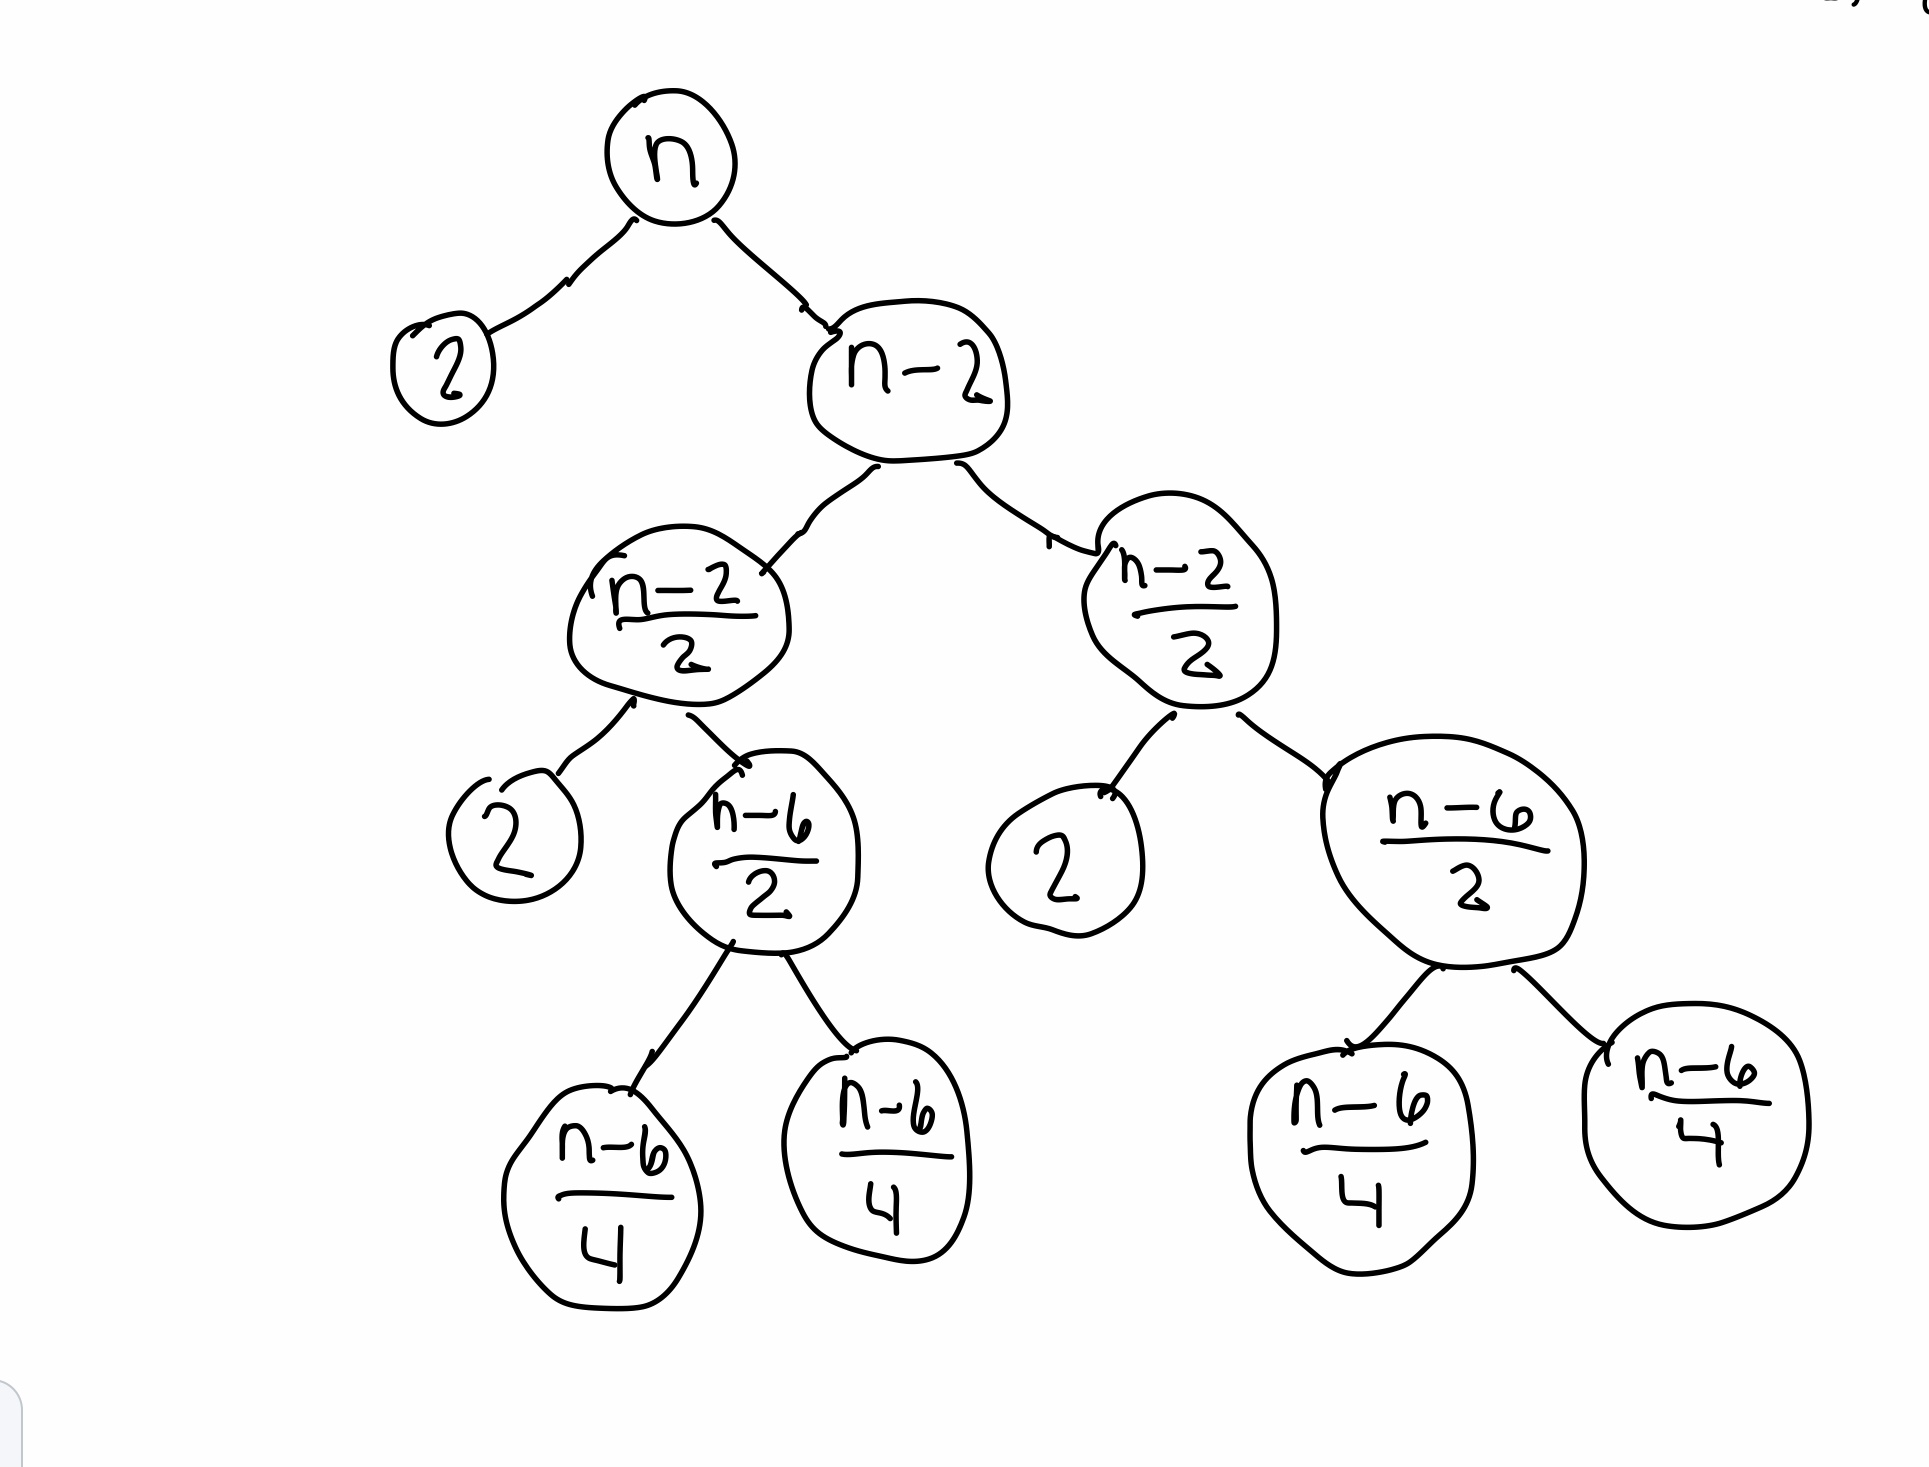
\includegraphics[width=0.5\textwidth]{1c1Hw6} \\

I will now examine every other level of the tree to identify the base case \\
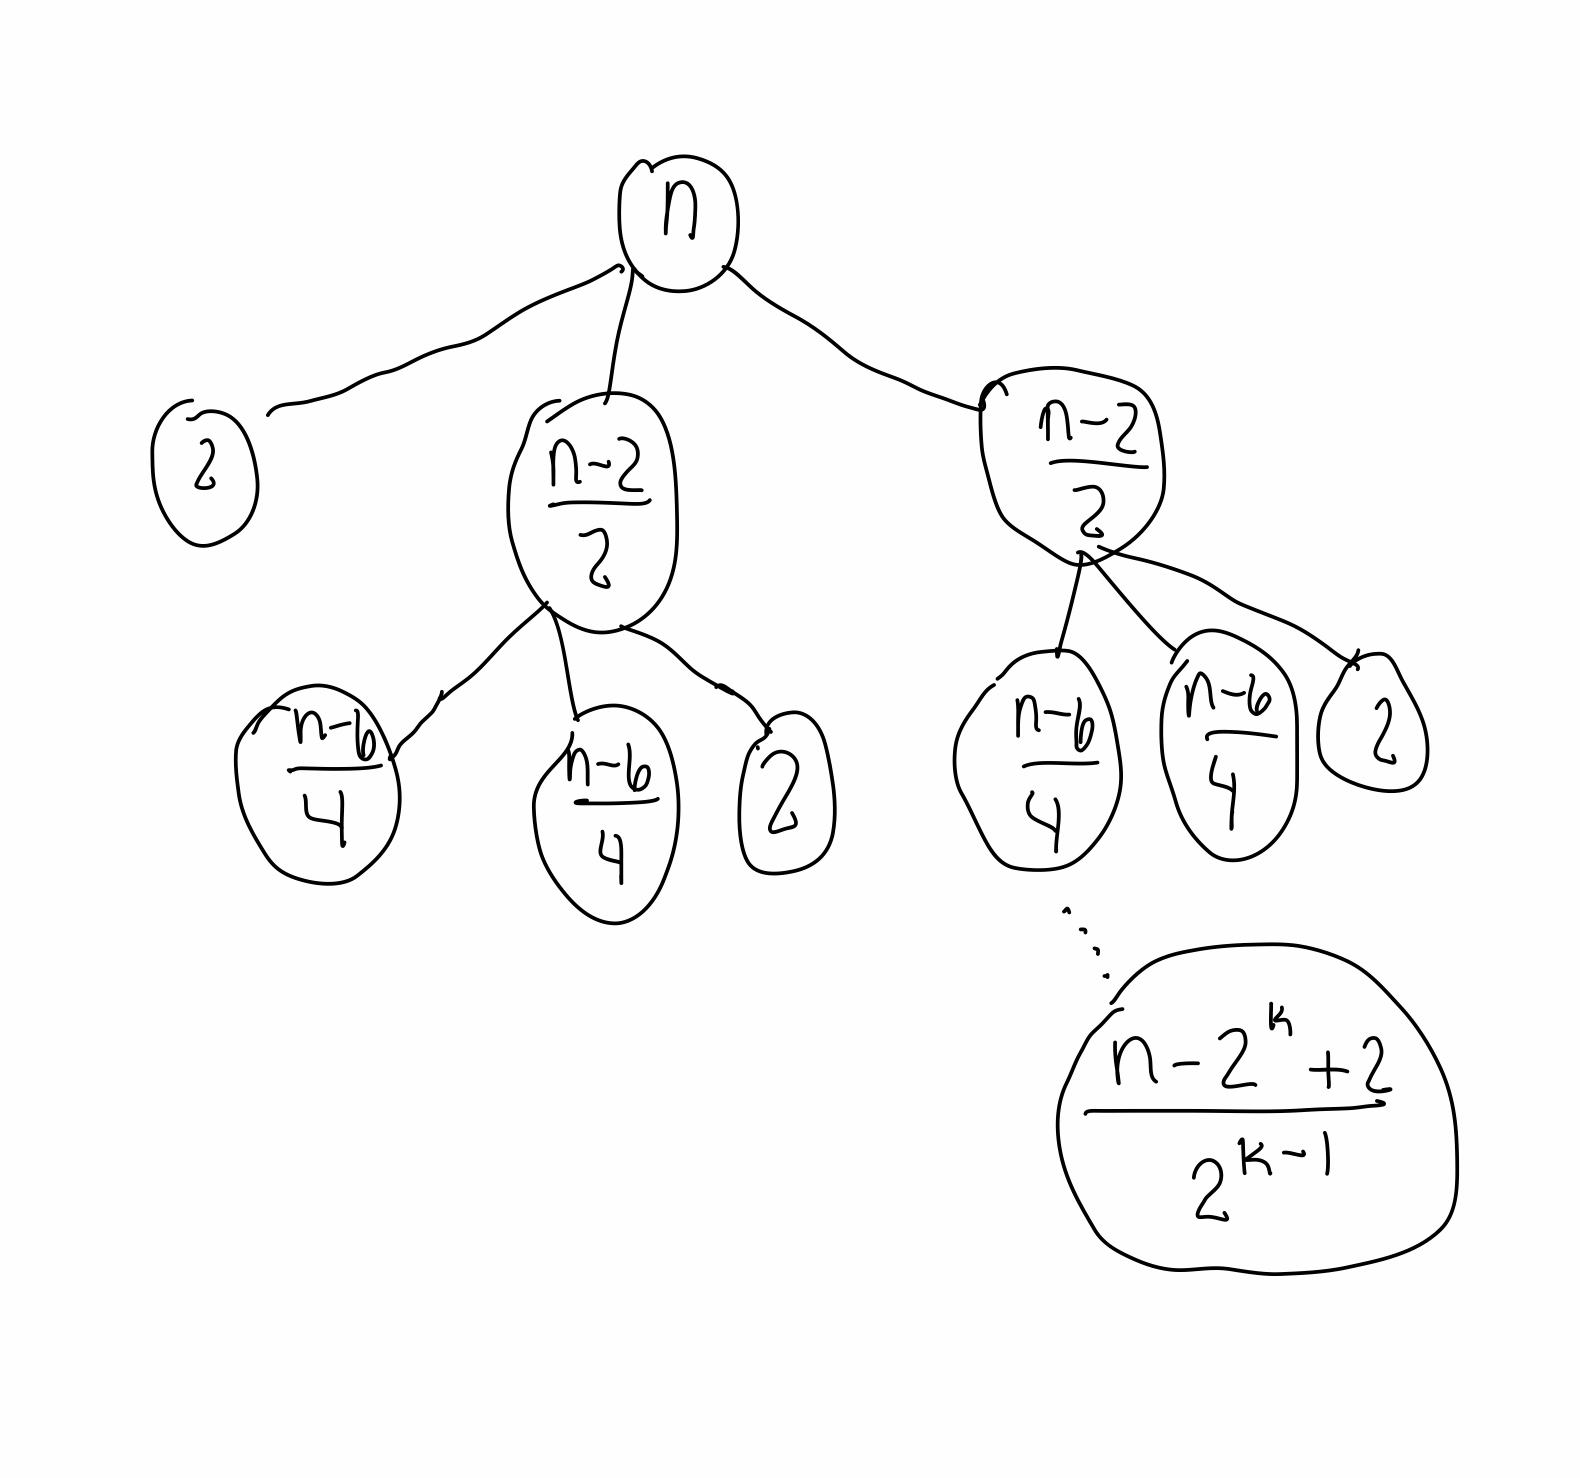
\includegraphics[width=0.5\textwidth]{1c2Hw6} \\


Observe that at level i of the tree the amount of nonrecursive work is $2\cdot(n-2^i+2) = 2(n+2)-2\cdot2^i$

Let us now determine the number of levels of the tree. Let k denote the number of levels of the tree. We will solve for k. The leaf nodes correspond to the base cases. 
We hit base cases when $\frac{n-2^k+2}{2^{k-1}} \leq  2$ \\ 
Solving for k we get $log_2(n+2)-1 \leq k$ \\
So the number of levels of the tree is $k = \lceil log_2(n+2)-1 \rceil$ \\

So the total work is \\
\begin{align*}
T(n) &\leq \sum_{i=0}^{\lceil log_2(n+2)-1 \rceil}(2(n+2)-2\cdot2^i)\\
 &\leq 2(n+2) \sum_{i=0}^{\lceil log_2(n+2)-1 \rceil}(1) - 2 \cdot \sum_{i=0}^{\lceil log_2(n+2)-1 \rceil}(2^i) \\
 &\leq 2(n+2)\cdot(\lceil log_2(n+2)-1 \rceil )- 2 \cdot \frac{(n+2)}{2} \\
 &\leq 2(n+2)\cdot(\lceil log_2(n+2)-1 \rceil )- (n+2) \\
\end{align*}

Thus, we have that $T(n) \in O(nlogn)$
.
Thus, this merge sort algorithm does not signicicantly change the running time of merge sort, as traditional merge sort is $T(n) \in \Theta(nlogn)$ 
\end{proof}

\end{enumerate}
\end{required}


\newpage
\section{Standard 18: Quicksort.}

\subsection{Problem 2}
\begin{required}
Given an input array $\{3,~7,~1,~8,~2,~6,~5,~4\}$. Consider the deterministic QuickSort algorithm and show the input array, the output array, and the global array at every partition as in the example in Section 2.1.1 of the course notes for week 8 (see Week 8 under ``Modules" of the course canvas). 

\begin{proof}[Answer]
% YOUR ANSWER HERE
\begin{tabular}{lll | ll}

procedure  &  arguments  &  input  &  output  &  global array  \\
\hline
first partition &  x=4, p=0, r=7  &  A=[3,7,1,8,2,6,5,4]  & A=[3,1,2, \textbf{4}, 7, 6, 5, 8] &  A=[3,1,2, 4, 7, 6, 5, 8] \\
\\
LQuicksort \\ partition & x=2, p=0, r=2 &  A=[3,1,\textbf{2}]  & A=[1, \textbf{2}, 3]  &  A=[1, 2, 3, 4, 7 ,6, 5, 8] \\
\\
RQuicksort \\partition(A,4,7) &  x=8, p=4, r=7  &  A=[7,6,5,\textbf{8}]  &  A=[7,6,5,\textbf{8}]  &  A=[1, 2, 3, 4, 7 ,6, 5, 8] \\
\\
L(LQuicksort) \\ partition & do nothing &    &  &  A=[1, 2, 3, 4, 7 ,6, 5, 8] \\
\\
L(RQuicksort) \\ partition & do nothing &    &  &  A=[1, 2, 3, 4, 7 ,6, 5, 8] \\
\\
R(LQuicksort) \\ partition &  x=5, p=4, r=6  &  A=[7,6,\textbf{5}]  &  A=[\textbf{5},6,7]  &  A=[1, 2, 3, 4, 5 ,6, 7, 8]  \\
\\
R(RQuicksort) \\ partition & do nothing &  &    &  A=[1, 2, 3, 4, 5 ,6, 7, 8]  \\
\\
RL(LQuicksort) \\ partition & do nothing &  &    &  A=[1, 2, 3, 4, 5 ,6, 7, 8]  \\
\\
RL(RQuicksort) \\ partition &  x=7, p=5, r=6  &  A=[6,\textbf{7}]  &  No change A=[6,\textbf{7}]  &  A=[1, 2, 3, 4, 5 ,6, 7, 8]  \\

RLR(LQuicksort) \\ partition & do nothing &  &    &  A=[1, 2, 3, 4, 5 ,6, 7, 8]  \\
\\
RLR(RQuicksort) \\ partition & do nothing &  &    &  A=[1, 2, 3, 4, 5 ,6, 7, 8]  \\
\\


\end{tabular}

\end{proof}

\end{required}

\newpage
\subsection{Problem 3}
\begin{required}

Suppose that we modify {\sc Partition}($A,s,e$) so that it chooses the median element of $A[s..e]$ in calls that occur in nodes of even depth of the recursion tree of a call {\sc Quicksort}($A[1, \ldots, n],1, n$), and it chooses the minimum element of $A[s..e]$ in calls that occur in nodes of odd depth of this recursion tree. \\
  
\noindent Assume that the running time of this modified {\sc Partition} is still $\Theta(n)$ on any subarray of length $n$. You may assume that the root of a recursion tree starts at level $0$ (which is an even number), its children are at level 1, etc. \\
  
\noindent Write down a recurrence relation for the running time of this version of {\sc Quicksort} given an array $n$ distinct elements and solve it asymptotically, i.e.\ give your answer as $\Theta(f(n))$ for some function $f(n)$. Show your work.

\begin{proof}[Answer]
% YOUR ANSWER HERE
The recurrences are \\
\begin{align*}
T_1(n) = \begin{cases}
\Theta(1) & : n \leq 2, \\
T_2(n-1) + 1+ \Theta(n) & : n > 2.
\end{cases}
\end{align*}
\begin{align*}
T_2(n) = \begin{cases}
\Theta(1) & : n \leq 2, \\
2T_1(\frac{n}{2}) + \Theta(n) & : n > 2.
\end{cases}
\end{align*}

The tree is below: \\
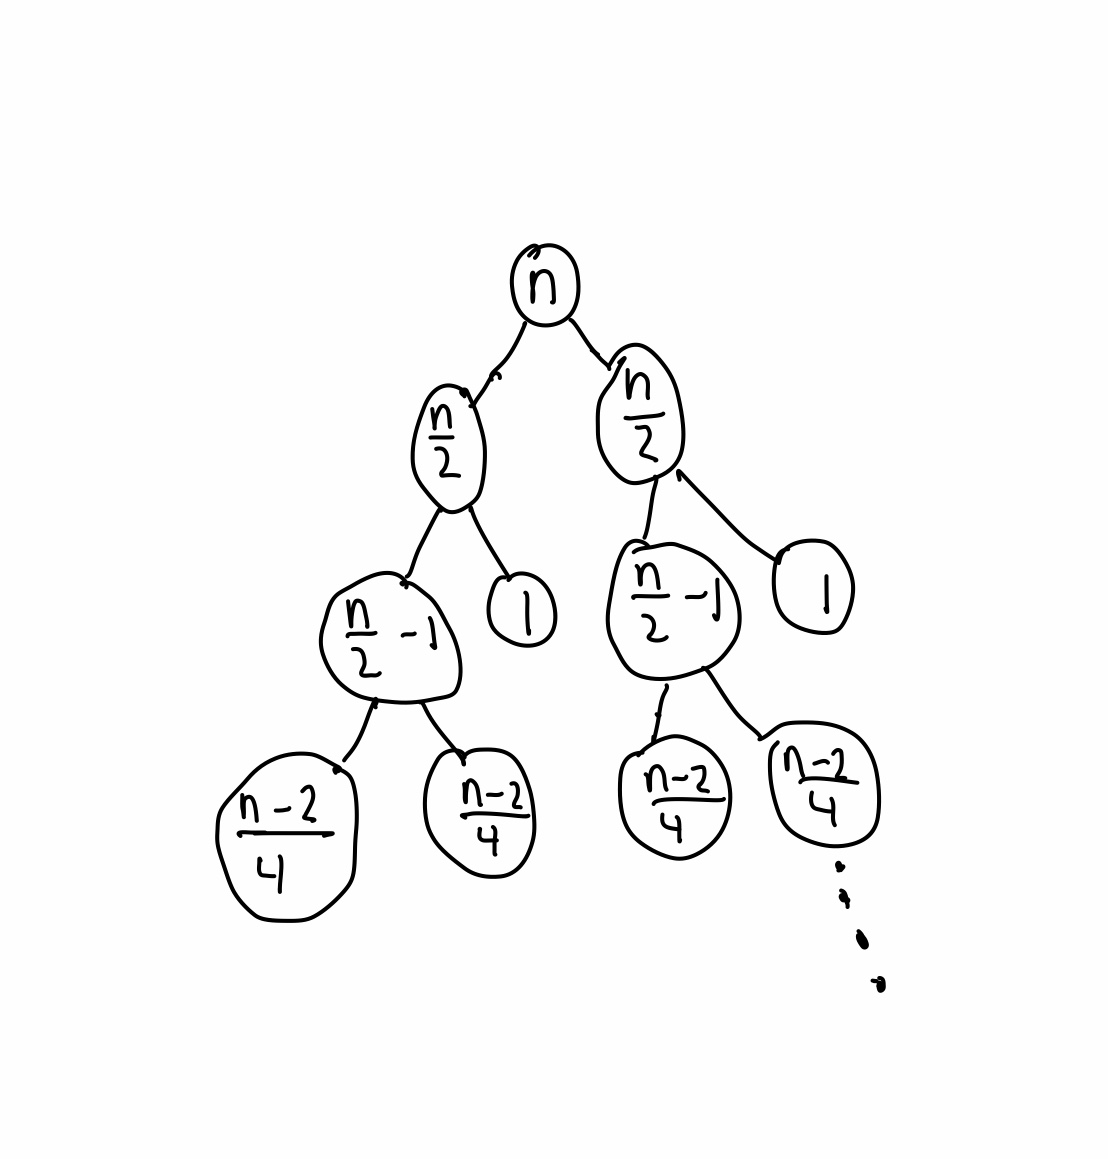
\includegraphics[width=0.5\textwidth]{Hw6Q3} \\

Observe that at level i of the tree the amount of nonrecursive work is $c(\frac{n}{2^i})$ and there are $2^i$ nodes at level $i$ \\
So the nonrecursive work at level $i$ is : $c(\frac{n}{2^i})\cdot 2^i= cn$ \\

Let us now determine the number of levels of the tree. Let k denote the number of levels of the tree. We will solve for k. The leaf nodes correspond to the base cases. 
We hit base cases when $\frac{n}{2^k} \leq  2$ \\ 
Solving for k we get $log_2n-1 \leq k$ \\
So the number of levels of the tree is $k = \lceil log_2(n)-1\rceil$ \\

So the total work is \\
\begin{align*}
T(n) &\leq \sum_{i=0}^{\lceil log_2(n)-1\rceil}(cn)\\
&\leq cn\cdot \lceil log_2(n)-1\rceil \\
\end{align*}

Thus, we have that $T(n) \in O(nlogn)$

\end{proof}

\end{required}

\end{document} % NOTHING AFTER THIS LINE IS PART OF THE DOCUMENT